
\labday{Mardi, 5 avril 2016}

Expérimentation sur le correcteur. Je vais résumé ici mes résultats et remarques
sur l'utilisation d'un correcteur simple (une seule couche) pour apprendre par l'exemple
à inverser des transformations linéaires simples.

Pour ce j'utilise le modèle simpliste (figure \ref{fig:correcteur}). 
Sans utilisation d'adversarial.

\begin{figure}[H]
\centering
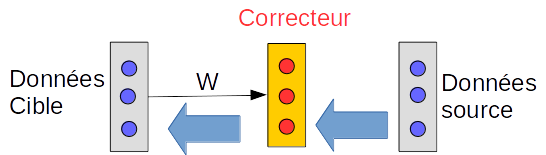
\includegraphics[width=0.45\linewidth]{fig/05-04-2016/Correcteur.png}
\caption{Correcteur simple}
\label{fig:correcteur}
\end{figure}

Le réseau est entraîné par minibatch avec un nombre d'époque prédéfini à la main.
La fonction de coût utilisée est la \emph{mean squared error} : $(\pmb{x_{pred}}-\pmb{x_{vrai}})^2$

Puisqu'il n'y a pas de \emph{décodeur} l'unique couche (unique matrice de poids $W$)
est constituée de $d$ neurone où $d$ est le nombre de descripteur des données.

\textbf{Remarque:} Les données ont été séparées en 3:
\begin{itemize}
	\item Les données d'\emph{entraînement} (très grosse majorité des données)
	\item Les données de \emph{validation} qui sont utilisées dans les courbes 
	d'apprentissages et qui servent de mesure pour l'optimisation (à la main) des 
	hyper-paramètres.
	\item Les données de \emph{test} qui servent à la visualisation des données (ne 
	sont utilisées ni pendant l'entraînement ni pendant la recherche d'un jeu de paramètre 
	donnant des résultats convenables).
\end{itemize}


\experiment{Corriger MNIST après transformations linéaires}

Dans un premier temps sur MNIST.
Le réseaux doit reconstruire l'image transformée.
MNIST est assez pratique car il permet de visualiser facilement l'efficacité 
de la reconstruction pour des données avec un bon nombre de descripteurs (748 pixels).

\subexperiment{Alignées}

Tout d'abord j'ai gardé la correspondance entre l'image original et
l'image transformée pendant l'entraînement du correcteur (cas aligné).
Ainsi chaque paire d'exemple $(\pmb{x}, \phi(\pmb{x})) \in MNIST\times \phi(MNIST)$
contient uniquement l'information que l'on cherche $\phi$.

Ce qui donne de très bon résultats la plupart du temps.\\


{\Large\textbf{Mirror.}} On commence par une simple permutation des 
descripteurs de façon à renverser les images.

Le correcteur se débrouille sans souci, sans avoir besoin d'adversarial. Ceci
nous offre un exemple typique de cas où tout se passe bien. Les résultats sont résumés
figure \ref{fig:mnist_mirror_pairwise}.

\begin{figure}[H] % Example of including images
\centering
\subfigure[Sample images]
	{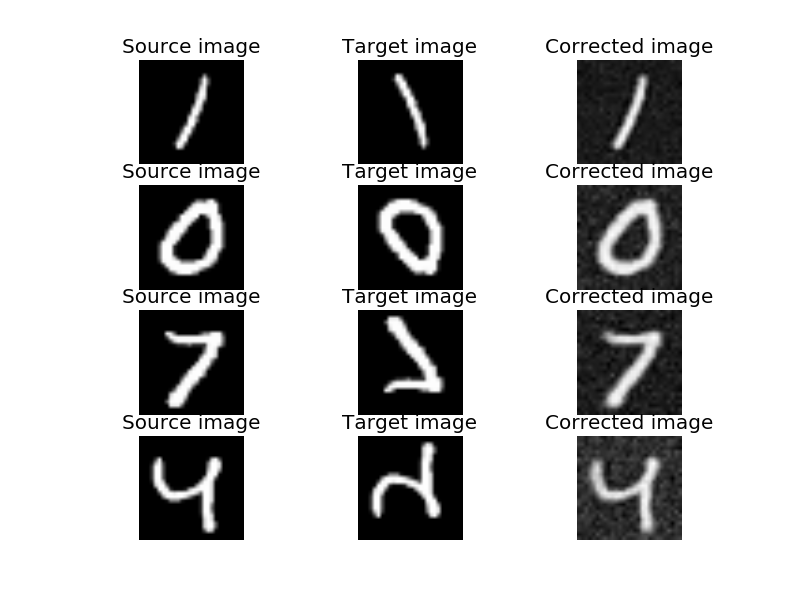
\includegraphics[width=0.45\linewidth]{fig/05-04-2016/MNISTMirror-PairWiseCorrector-lambda-0.0000-sample.png}}
\hfill
\subfigure[Learning curve (squared loss)]
	{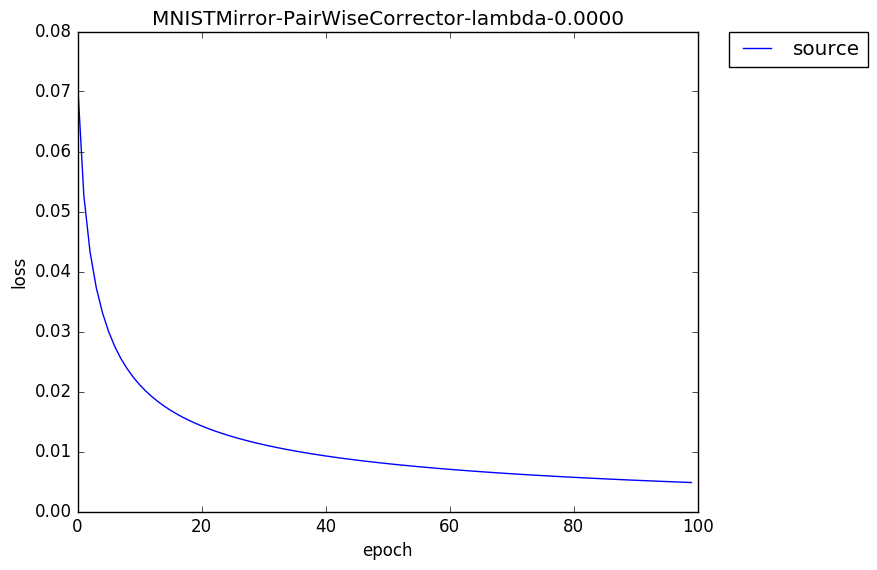
\includegraphics[width=0.45\linewidth]{fig/05-04-2016/MNISTMirror-PairWiseCorrector-lambda-0.0000.png}}
\subfigure[Weights]
	{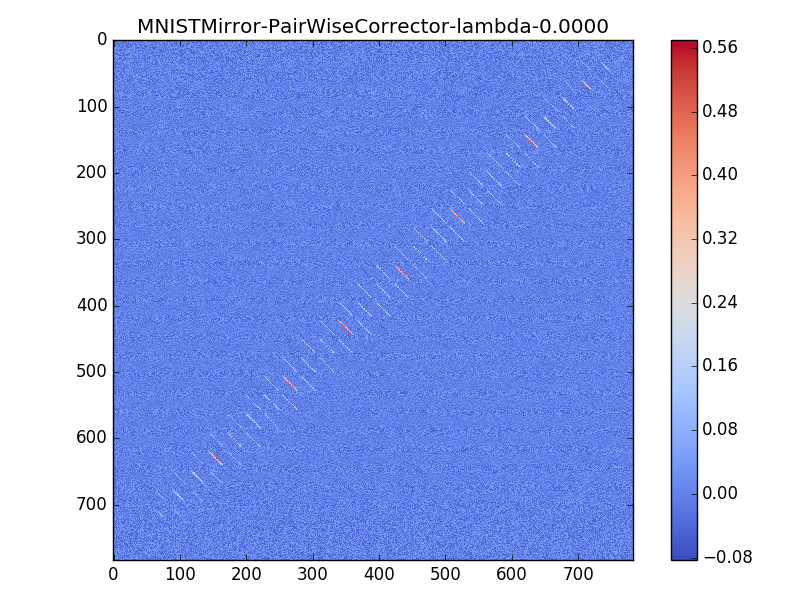
\includegraphics[width=0.45\linewidth]{fig/05-04-2016/MNISTMirror-PairWiseCorrector-lambda-0.0000-Weights.png}}
\caption{MNIST - Mirror correcteur aligné}
\label{fig:mnist_mirror_pairwise}
\end{figure}


{\Large\textbf{RMat.}} On se lance maintenant dans un problème légèrement plus
difficile pour la machine mais impossible pour l'œil humain, une transformation
linéaire aléatoire:
$$ \phi(\pmb{x}) = A.\pmb{x}$$
où $A$ est une matrice générée aléatoirement.

Pour éviter les problèmes d'échelle, les données ont été renormalisées après 
transformation (sinon : loss = NaN).

Les résultats sur cette transformation sont assez mitigés. De plus elle requiert
un entraînement particulièrement long (quelques centaines d'époques). Mais bon avec
les yeux de la fois et en choisissant les bons exemples ça a l'air de fonctionner.
Une fois de plus les résultats sont résumés figure \ref{fig:mnist_rmat_pairwise}.

\begin{figure}[H] % Example of including images
\centering
\subfigure[Sample images]
	{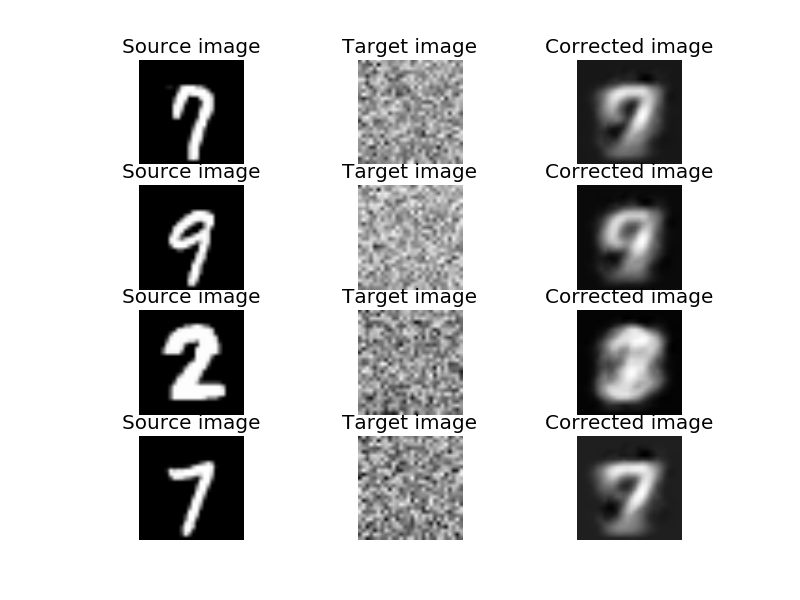
\includegraphics[width=0.45\linewidth]{fig/05-04-2016/MNISTRMat-PairWiseCorrector-lambda-0.0000-sample.png}}
\hfill
\subfigure[Learning curve (squared loss)]
	{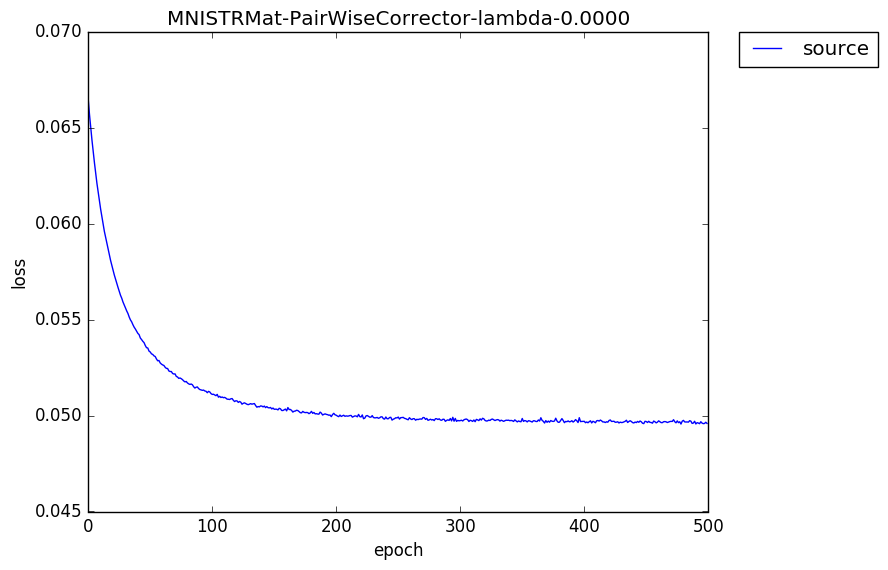
\includegraphics[width=0.45\linewidth]{fig/05-04-2016/MNISTRMat-PairWiseCorrector-lambda-0.0000.png}}
\subfigure[Weights]
	{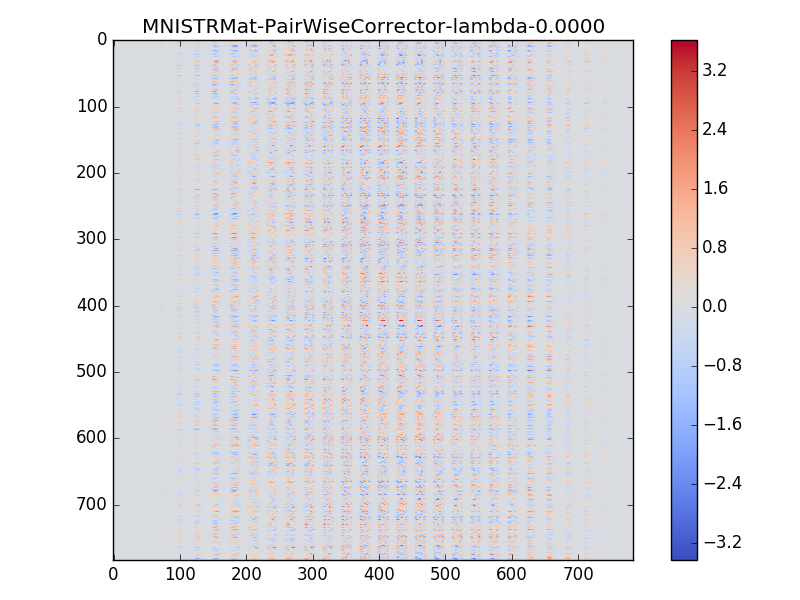
\includegraphics[width=0.45\linewidth]{fig/05-04-2016/MNISTRMat-PairWiseCorrector-lambda-0.0000-Weights.png}}
\caption{MNIST - RMat correcteur aligné}
\label{fig:mnist_rmat_pairwise}
\end{figure}


\subexperiment{Non alignées}

Ici chaque paire d'exemple $(\pmb{x_i}, \phi(\pmb{x_j})) \in MNIST\times \phi(MNIST)$
ne contient pas uniquement l'information que l'on cherche $\phi$. Même si
les exemples $\pmb{x_i}$ et $\pmb{x_j}$ sont choisis parmi la même classe
$y_i=y_j$, ces exemples se différencient non seulement par la transformation 
subie mais aussi par les variations au sein d'une même classes.

Ceci est plus proche de cas d'expériences réelles. Exemple: des échantillons
du même type sans être exactement les mêmes et utilisant des instruments
de précision différentes.

L'entraînement est donc légèrement plus complexe. Pour le moment j'ai utilisé 
la version naïve où je sélectionne aléatoirement les exemples d'une même classe
pour être alignés. Cette sélection change à chaque nouvelle époque. Des 
améliorations possibles de cette technique seront développées plus loin
(section \ref{exp:amelioration_0}).\\


{\Large\textbf{Mirror.}} à nouveau l'on commence par le cas simple des images 
miroirs. Cette fois ci la qualité des résultats est plus discutable. 

\begin{figure}[H] % Example of including images
\centering
\subfigure[Sample images]
	{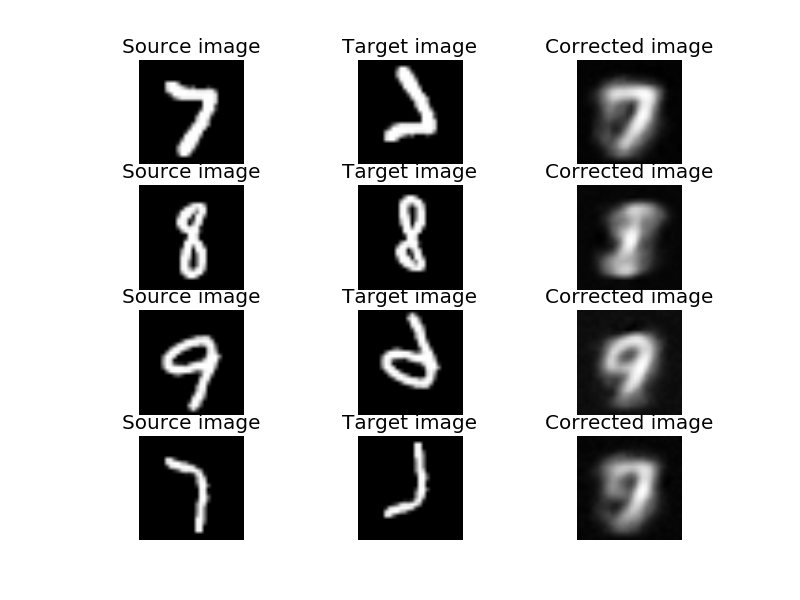
\includegraphics[width=0.45\linewidth]{fig/05-04-2016/MNISTMirror-ClassWiseCorrector-lambda-0.0000-sample.png}}
\hfill
\subfigure[Learning curve (squared loss)]
	{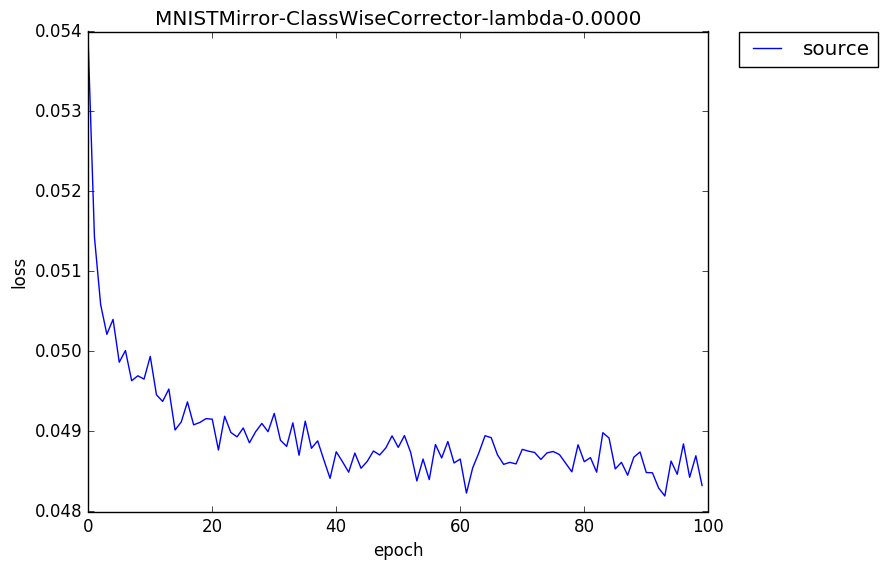
\includegraphics[width=0.45\linewidth]{fig/05-04-2016/MNISTMirror-ClassWiseCorrector-lambda-0.0000.png}}
\subfigure[Weights]
	{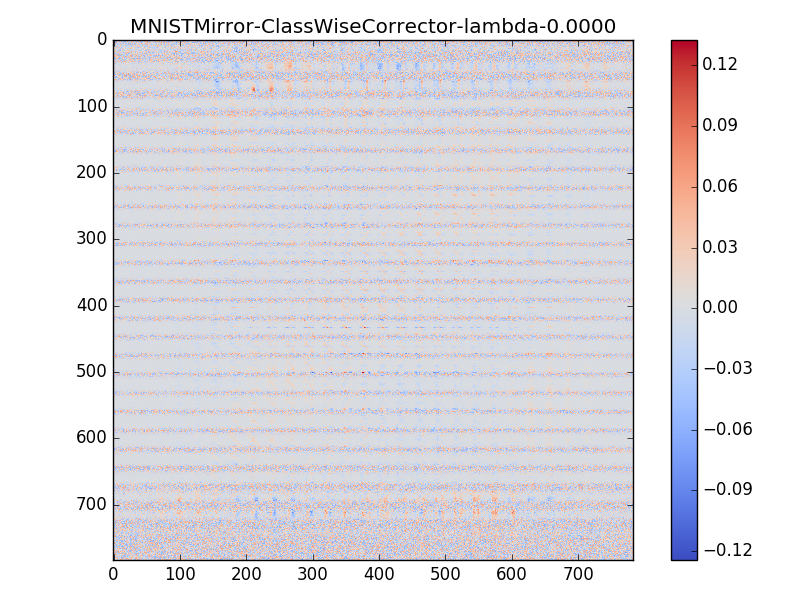
\includegraphics[width=0.45\linewidth]{fig/05-04-2016/MNISTMirror-ClassWiseCorrector-lambda-0.0000-Weights.png}}
\caption{MNIST - Mirror correcteur non aligné}
\label{fig:mnist_mirror_classwise}
\end{figure}


{\Large\textbf{RMat.}} On reprend la transformation linéaire aléatoire:
$$ \phi(\pmb{x}) = A.\pmb{x}$$
où $A$ est une matrice générée aléatoirement.


\begin{figure}[H] % Example of including images
\centering
\subfigure[Sample images]
	{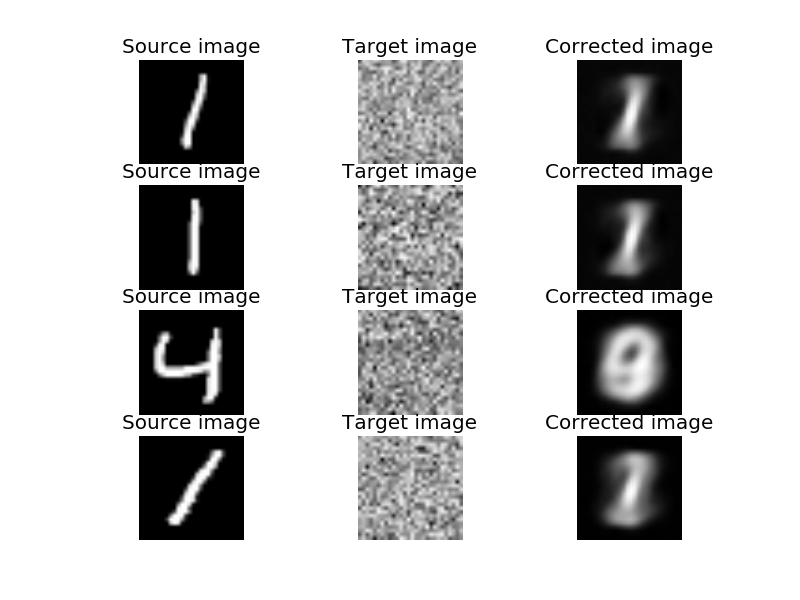
\includegraphics[width=0.45\linewidth]{fig/05-04-2016/MNISTRMat-ClassWiseCorrector-lambda-0.0000-sample.png}}
\hfill
\subfigure[Learning curve (squared loss)]
	{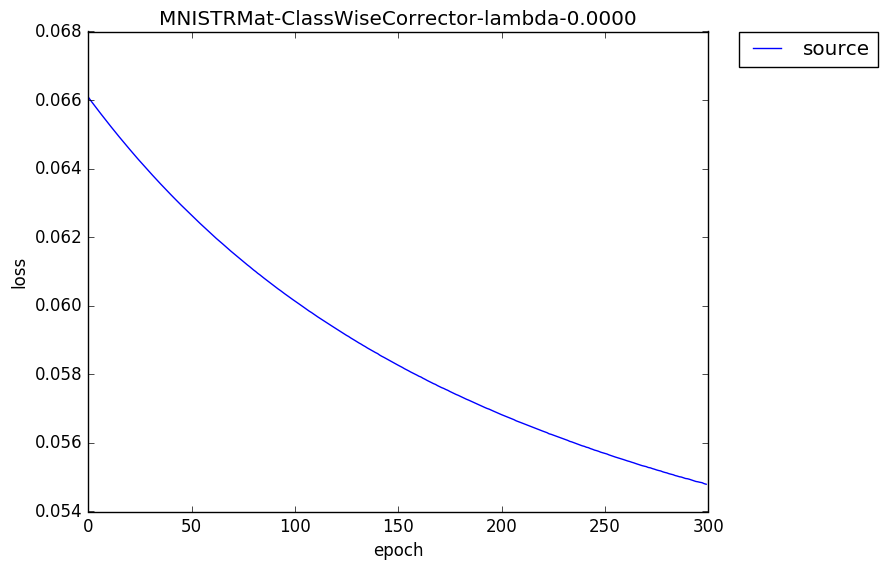
\includegraphics[width=0.45\linewidth]{fig/05-04-2016/MNISTRMat-ClassWiseCorrector-lambda-0.0000.png}}
\subfigure[Weights]
	{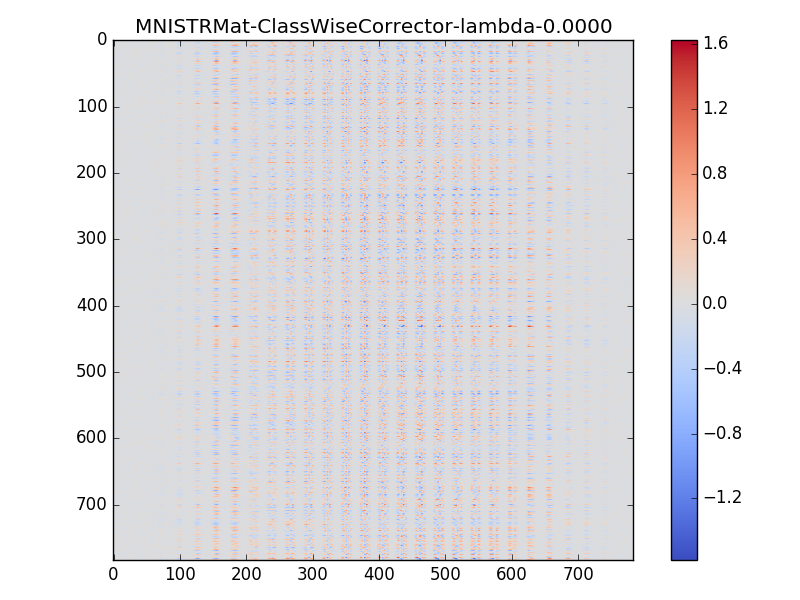
\includegraphics[width=0.45\linewidth]{fig/05-04-2016/MNISTRMat-ClassWiseCorrector-lambda-0.0000-Weights.png}}
\caption{MNIST - RMat correcteur non aligné}
\label{fig:mnist_rmat_classwise}
\end{figure}


%-----------------------------------------

\experiment{Corriger Moon après transformations linéaire}

Maintenant on passe sur des données à 2 dimensions. L'exemple des demi-lunes
(Moon) est un exemple non linéaire simple en 2D.\\

\subexperiment{Alignées}

Tout d'abord j'ai gardé la correspondance entre les points originaux et
les points transformées pendant l'entraînement du correcteur (cas aligné).
Ainsi chaque paire d'exemple $(\pmb{x}, \phi(\pmb{x})) \in Moon\times \phi(Moon)$
contient uniquement l'information que l'on cherche $\phi$.

Ce qui donne de très bon résultats.\\


{\Large\textbf{Rotated.}} On commence avec une rotation ie :
$$ \phi(\pmb{x}) = R.\pmb{x}$$
où $R$ est une matrice de rotation.

Les résultats sont parfaits. Comme on peut le remarquer figure 
\ref{fig:moon_rotated_pairwise} les croix (données corrigées) tombent toutes
dans les ronds (données sources).

\begin{figure}[H] % Example of including images
\centering
\subfigure[Sample images]
	{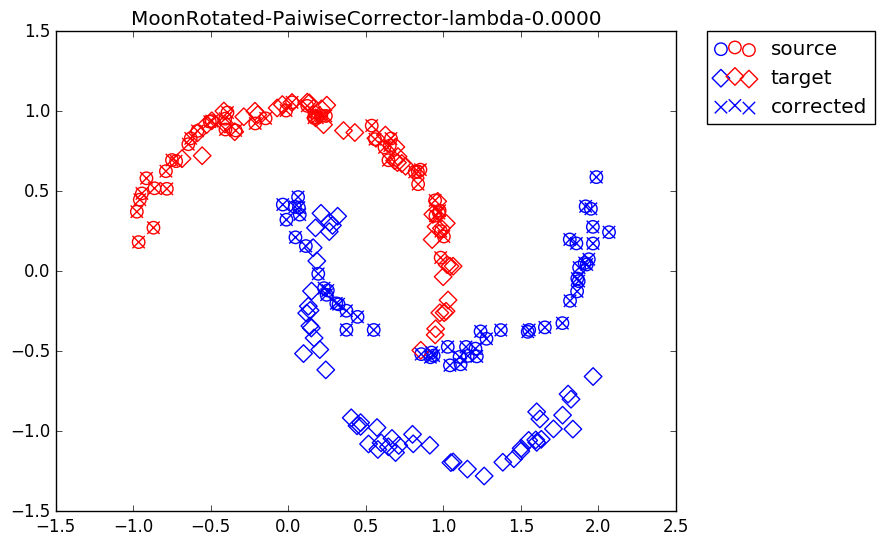
\includegraphics[width=0.45\linewidth]{fig/05-04-2016/MoonRotated-PaiwiseCorrector-lambda-0.0000-data.png}}
\hfill
\subfigure[Learning curve (squared loss)]
	{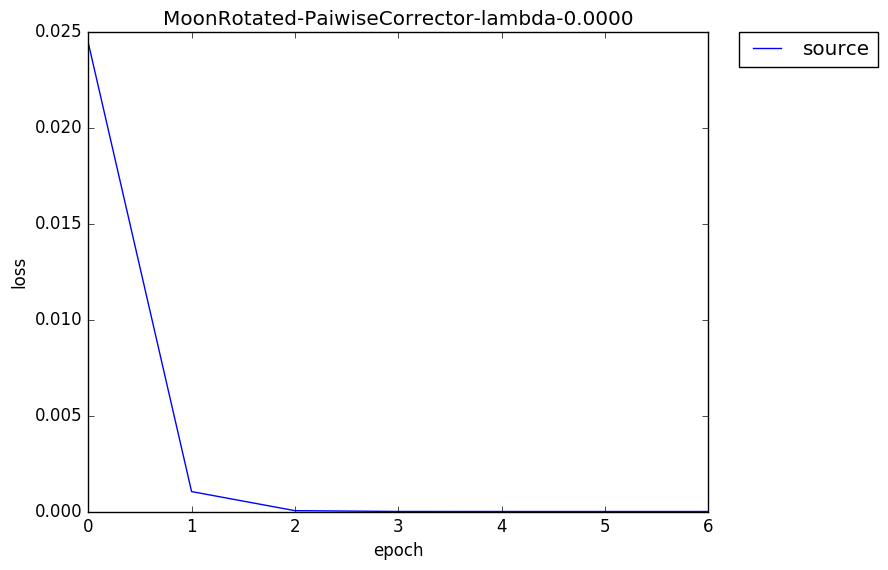
\includegraphics[width=0.45\linewidth]{fig/05-04-2016/MoonRotated-PaiwiseCorrector-lambda-0.0000.png}}
\caption{Moon - Rotated correcteur aligné}
\label{fig:moon_rotated_pairwise}
\end{figure}


{\Large\textbf{RMat.}} On se lance alors dans les transformations linéaires aléatoires:
$$ \phi(\pmb{x}) = A.\pmb{x}$$
où $A$ est une matrice générée aléatoirement.

Ce qui donne un résultat identique (figure \ref{fig:moon_rmat_pairwise}).


\begin{figure}[H] % Example of including images
\centering
\subfigure[Sample images]
	{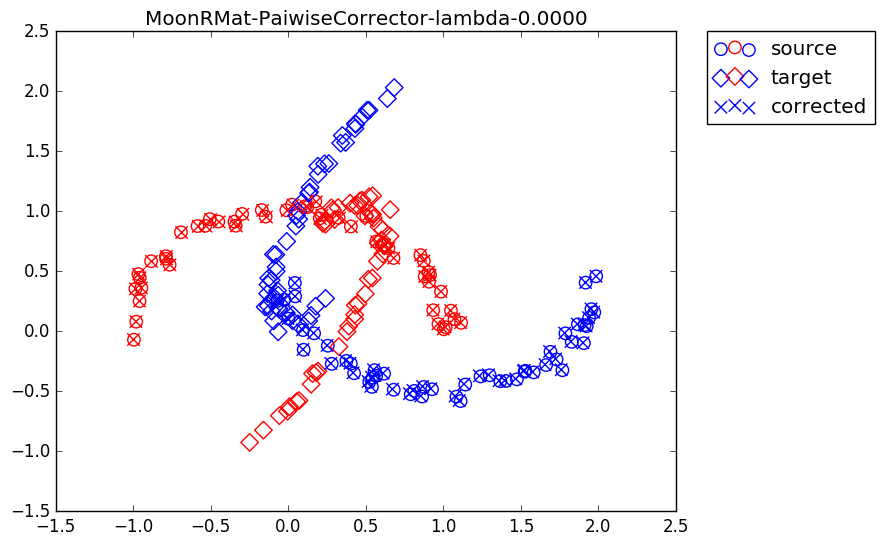
\includegraphics[width=0.45\linewidth]{fig/05-04-2016/MoonRMat-PaiwiseCorrector-lambda-0.0000-data.png}}
\hfill
\subfigure[Learning curve (squared loss)]
	{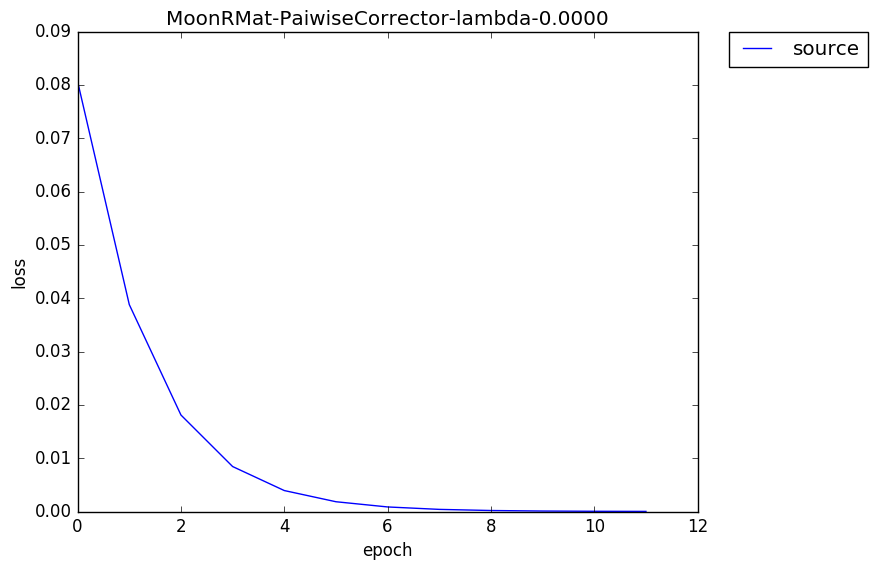
\includegraphics[width=0.45\linewidth]{fig/05-04-2016/MoonRMat-PaiwiseCorrector-lambda-0.0000.png}}
\caption{Moon - RMat correcteur aligné}
\label{fig:moon_rmat_pairwise}
\end{figure}



\subexperiment{Non alignées}

Ici chaque paire d'exemple $(\pmb{x_i}, \phi(\pmb{x_j})) \in Moon\times \phi(Moon)$
ne contient pas uniquement l'information que l'on cherche $\phi$. Même si
les exemples $\pmb{x_i}$ et $\pmb{x_j}$ sont choisis parmi la même classe
$y_i=y_j$, ces exemples se différencient non seulement par la transformation 
subie mais aussi par les variations au sein d'une même classes.

Ceci est plus proche de cas d'expériences réelles. Exemple: des échantillons
du même type sans être exactement les mêmes et utilisant des instruments
de précision différentes.

L'entraînement est donc légèrement plus complexe. Pour le moment j'ai utilisé 
la version naïve où je sélectionne aléatoirement les exemples d'une même classe
pour être alignés. Cette sélection change à chaque nouvelle époque. Des 
améliorations possibles de cette technique seront développées plus loin 
(section \ref{exp:amelioration_0}).\\



{\Large\textbf{Rotated.}} On commence avec une rotation ie :
$$ \phi(\pmb{x}) = R.\pmb{x}$$
où $R$ est une matrice de rotation.

Les résultats sont mauvais. Comme on peut le remarquer figure 
\ref{fig:moon_rotated_classwise}.

\begin{figure}[H] % Example of including images
\centering
\subfigure[Sample images]
	{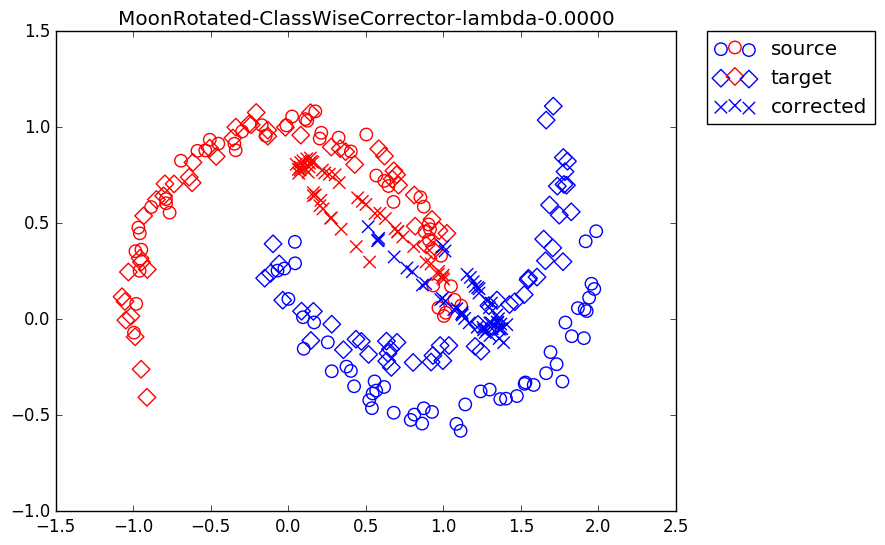
\includegraphics[width=0.45\linewidth]{fig/05-04-2016/MoonRotated-ClassWiseCorrector-lambda-0.0000-data.png}}
\hfill
\subfigure[Learning curve (squared loss)]
	{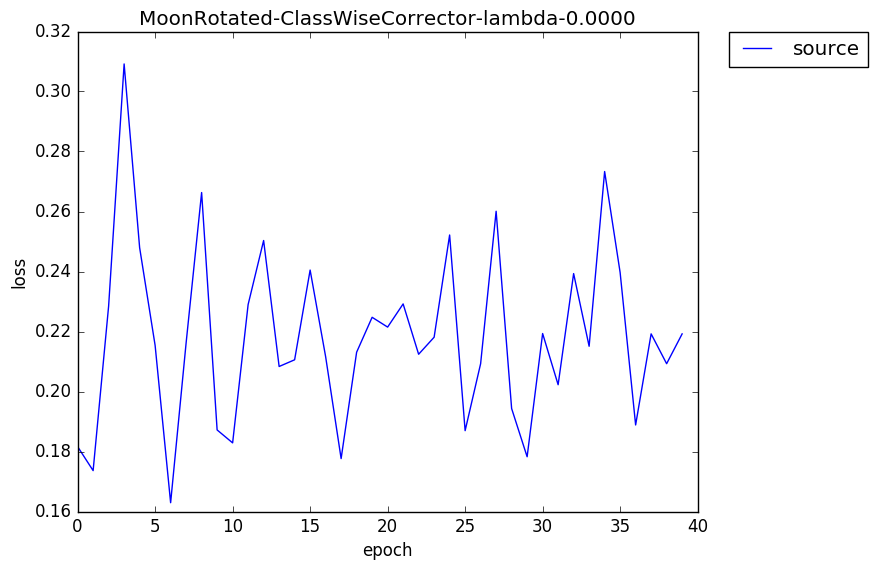
\includegraphics[width=0.45\linewidth]{fig/05-04-2016/MoonRotated-ClassWiseCorrector-lambda-0.0000.png}}
\caption{Moon - Rotated correcteur aligné}
\label{fig:moon_rotated_classwise}
\end{figure}


{\Large\textbf{RMat.}} On se lance alors dans les transformations linéaires aléatoires:
$$ \phi(\pmb{x}) = A.\pmb{x}$$
où $A$ est une matrice générée aléatoirement.

Ce qui donne un résultat identiquement mauvais (figure \ref{fig:moon_rmat_classwise}).


\begin{figure}[H] % Example of including images
\centering
\subfigure[Sample images]
	{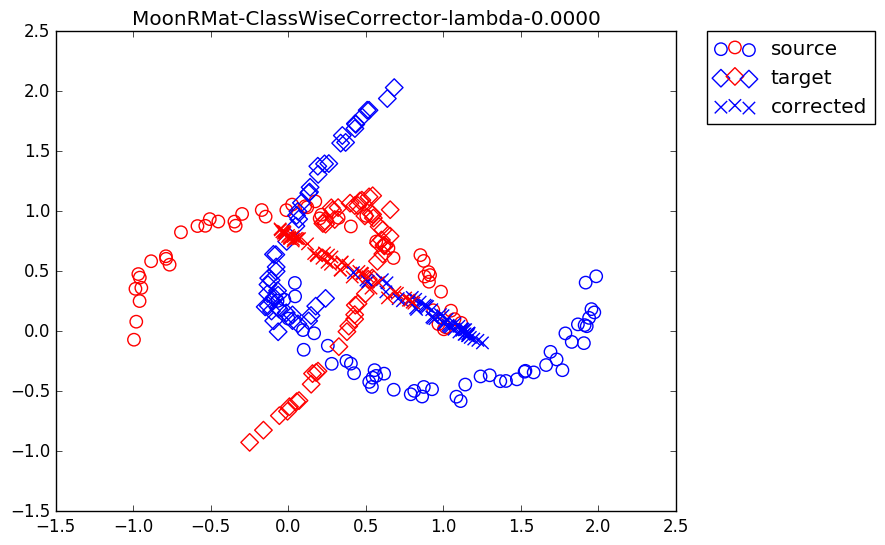
\includegraphics[width=0.45\linewidth]{fig/05-04-2016/MoonRMat-ClassWiseCorrector-lambda-0.0000-data.png}}
\hfill
\subfigure[Learning curve (squared loss)]
	{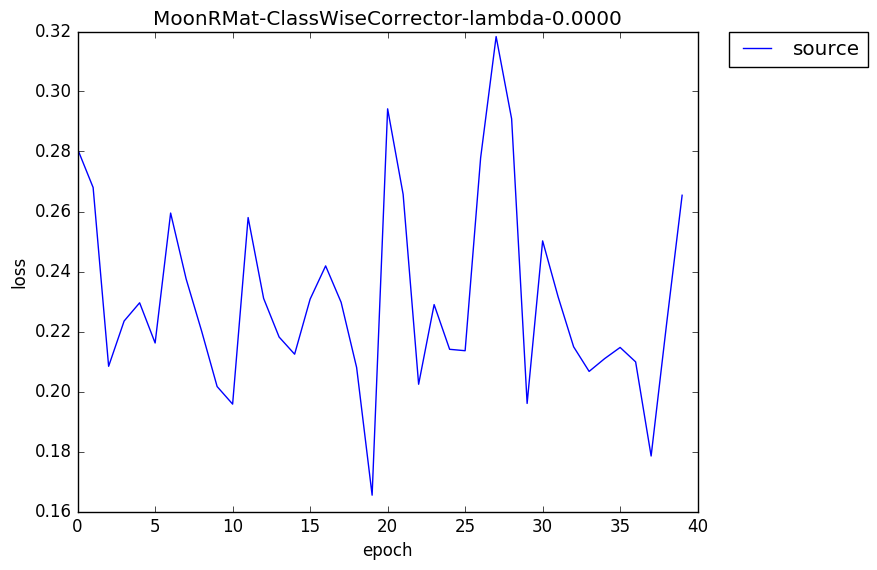
\includegraphics[width=0.45\linewidth]{fig/05-04-2016/MoonRMat-ClassWiseCorrector-lambda-0.0000.png}}
\caption{Moon - RMat correcteur aligné}
\label{fig:moon_rmat_classwise}
\end{figure}


\experiment{Amélioration}
\label{exp:amelioration_0}

Une des améliorations possibles utilise un entraînement alternatif entre la 
reconstruction et une branche adversariale (figure \ref{fig:correcteur_adversarial}).

\begin{figure}[H]
\centering
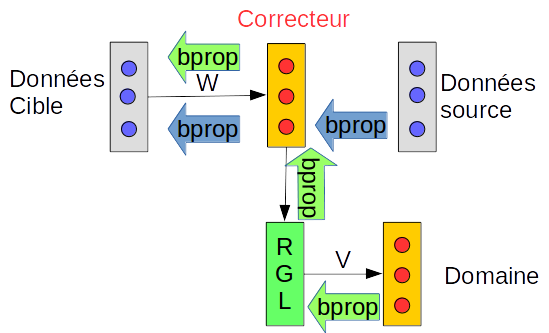
\includegraphics[width=0.45\linewidth]{fig/05-04-2016/Correcteur-Adversarial.png}
\caption{Correcteur adversarial}
\label{fig:correcteur_adversarial}
\end{figure}

Et je viens de m'apercevoir que mon implémentation ne fait pas ça ... Je fais 
passer les données sources dans le correcteur, ce qu'il ne faut PAS faire. 

%----------------------------------------------------------------------------------------
